\documentclass[doc,natbib,12pt]{article}

\usepackage[american]{babel}
\usepackage[utf8x]{inputenc}
\usepackage{amsmath}
\usepackage{graphicx}
\usepackage[colorinlistoftodos]{todonotes}
\usepackage{varioref}
\usepackage[hidelinks]{hyperref}
\usepackage[T1]{fontenc}

\title{CISC 611-90-O-2019/Late Spring - Network Operating Systems \\ Homework - 1}

\author{Youwei Lu}
\date{}

%\abstract{Referring to Operating Systems architecture, the topic of this assignment is on the ``Memory Management'' which is part of the computer's physical memory or Random-Access Memory (RAM) organization.}

\begin{document}
	\maketitle
	
	
	\section*{Problem 1. Given the following graph, use Dijkstra's shortest path algorithm to find shortest paths starting from node A. }
	
	\begin{figure}[htpb]
		\centering
		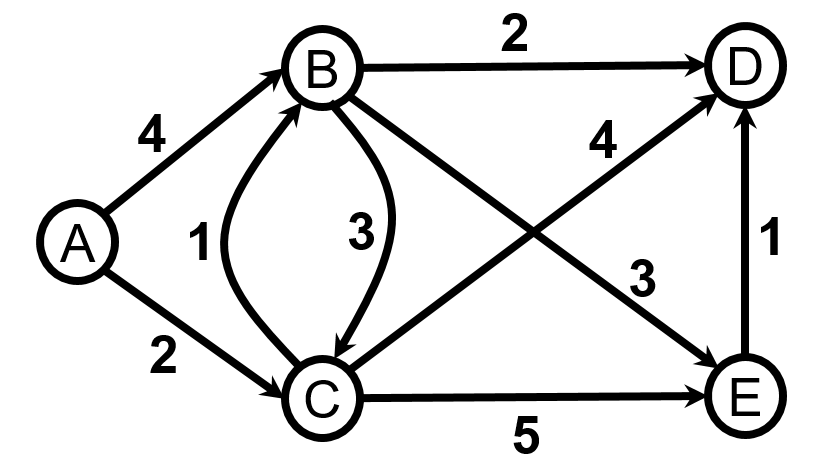
\includegraphics[width=0.5\textwidth]{1.png}
		\caption{\label{fig:problem1}Problem 1.}
	\end{figure}
	
	According to Dijkstra's algorithm, first we create a shortest path tree set that keeps track of all vertices included in the shortest path tree, and it can be used to mark the finalization of vertices one by one. The set is initially empty: \{null, null, null, null, null\}
	
	\subsection*{Step 1 to Problem 1}
	First pick A in the set, so that the distance from A is 0. The shortest path tree set is now: \{A, null, null, null, null\}, and the distance from A to B and C are 4 and 2, as shown in Figure~\ref{fig:problem1-step1}. Note that green color indicates the vertices have been chosen.
	
	\begin{figure}[htpb]
		\centering
		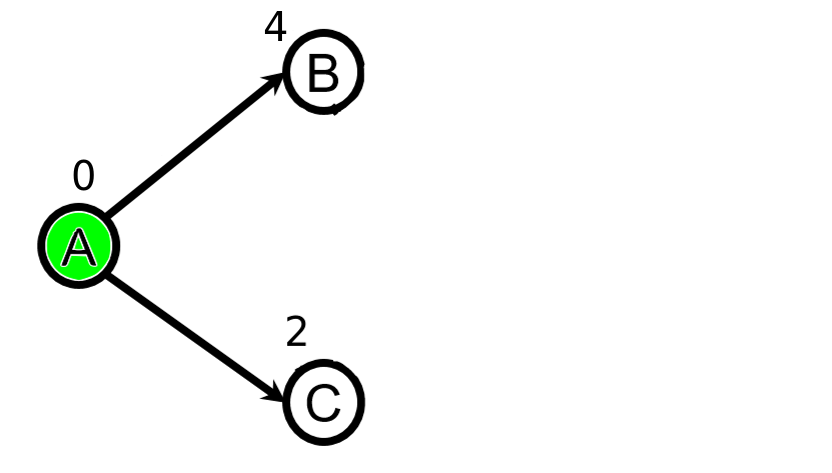
\includegraphics[width=0.5\textwidth]{1-1.png}
		\caption{\label{fig:problem1-step1}Step 1 to problem 1.}
	\end{figure}
	
	\subsection*{Step 2 to Problem 1}
	Since 2 is shorter than 4, vertex C is chosen. The shortest path tree set is now: \{A, C, null, null, null\}. The distance to B should be from A->C->B, which is 2 + 1 = 4, while the distance to D should be 2 + 4 = 6, and to E is 2 + 5 = 7. The choose and distances are shown in Figure~\ref{fig:problem1-step2}.
	
	\begin{figure}[htpb]
		\centering
		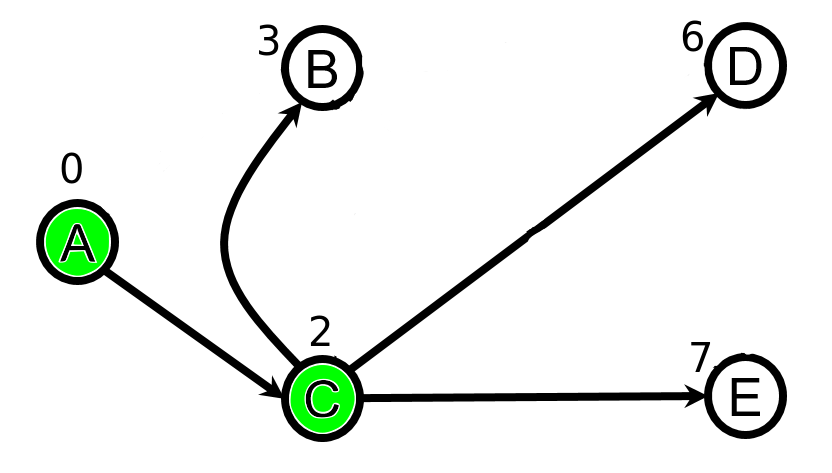
\includegraphics[width=0.5\textwidth]{1-2.png}
		\caption{\label{fig:problem1-step2}Step 2 to problem 1.}
	\end{figure}
	
	\subsection*{Step 3 to Problem 1}
	Since 3 is the shortest among the remaining distances, vertex B is chosen. The shortest path tree set is now: \{A, C, B, null, null\}. The distance to D and E now should be visited from B instead of C now. The distance to D is 3 + 2 = 5, and the distance to E is 3 + 3 = 6, as shown in Figure~\ref{fig:problem1-step3}.
	
	\begin{figure}[htpb]
		\centering
		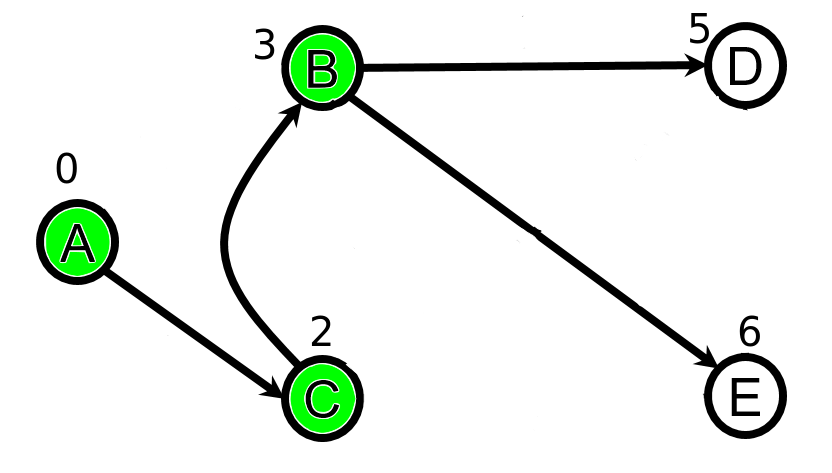
\includegraphics[width=0.5\textwidth]{1-3.png}
		\caption{\label{fig:problem1-step3}Step 3 to problem 1.}
	\end{figure}
	
	\subsection*{Step 4 to Problem 1}
	5 is shorter than 6, so D is chosen in this step. The shortest path tree set is now: \{A, C, B, D, null\}. As there's no path starting from D, the distance of E doesn't change, which is still from B, and still 6. See Figure~\ref{fig:problem1-step4}.
	
	\begin{figure}[htpb]
		\centering
		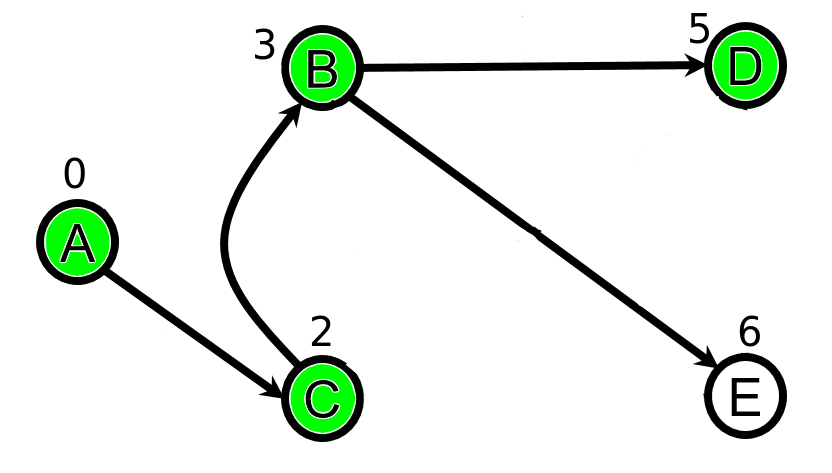
\includegraphics[width=0.5\textwidth]{1-4.png}
		\caption{\label{fig:problem1-step4}Step 4 to problem 1.}
	\end{figure}
	
	\subsection*{Step 5 to Problem 1}
	Choose the last vertex E, and the shortest path tree set is complete now: \{A, C, B, D, E\}. The final graph is shown in Figure~\ref{fig:problem1-step5}.
	
	\begin{figure}[htpb]
		\centering
		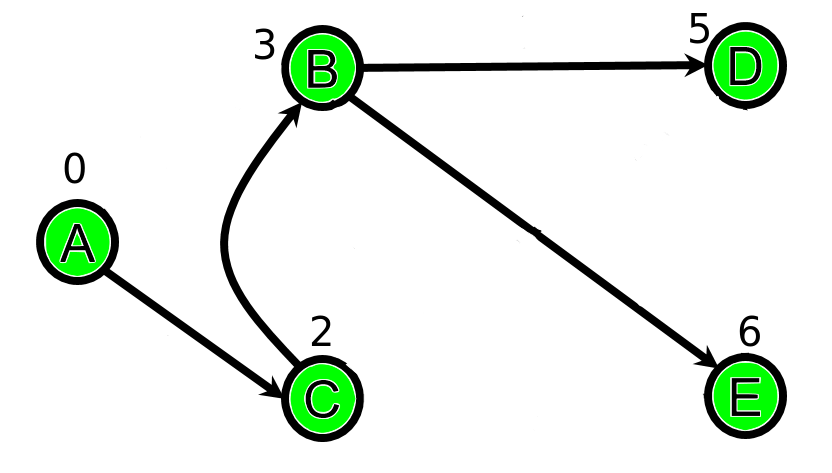
\includegraphics[width=0.5\textwidth]{1-5.png}
		\caption{\label{fig:problem1-step5}Step 5 (result) to problem 1.}
	\end{figure}
	
	\subsection*{Result to Problem 1}
	Steps to problem 1 can be summarized in Table~\ref{tab:problem1-result}. Note that bold text indicates the shortest distance in that step.
	
	\begin{table}[htpb]
		\centering
		\begin{tabular}{lllllll}
			Steps & Choose                 & A & B & C & D    & E    \\ \cline{1-7} 
			1 & \multicolumn{1}{l|}{A} & \textbf{0} & 4 & 2 & $\infty$ & $\infty$ \\
			2 & \multicolumn{1}{l|}{C} & \textbf{0} & 3 &\textbf{2} & 6    & 7    \\
			3 & \multicolumn{1}{l|}{B} & \textbf{0} & \textbf{3} & \textbf{2} & 5   & 6    \\
			4 & \multicolumn{1}{l|}{D} & \textbf{0} & \textbf{3} & \textbf{2} & \textbf{5}   &  6 \\
			5 & \multicolumn{1}{l|}{E} & \textbf{0} & \textbf{3} & \textbf{2} & \textbf{5}   &  \textbf{6}
		\end{tabular}
		\caption{\label{tab:problem1-result}Distances from A in problem 1.}
	\end{table}
	
	Figure~\ref{fig:problem1-step5} shows the shortest result graph to problem 1, and the shortest distances from A in problem 1 are \{A: 0, B: 3, C: 2, D: 5, E: 6\}.
	
	\section*{Problem 2. Given the following graph, can you still use Dijkstra's shortest path algorithm to find shortest paths from node S? If you cannot, try Bellman-Ford algorithm.}
	
	\begin{figure}[htpb]
		\centering
		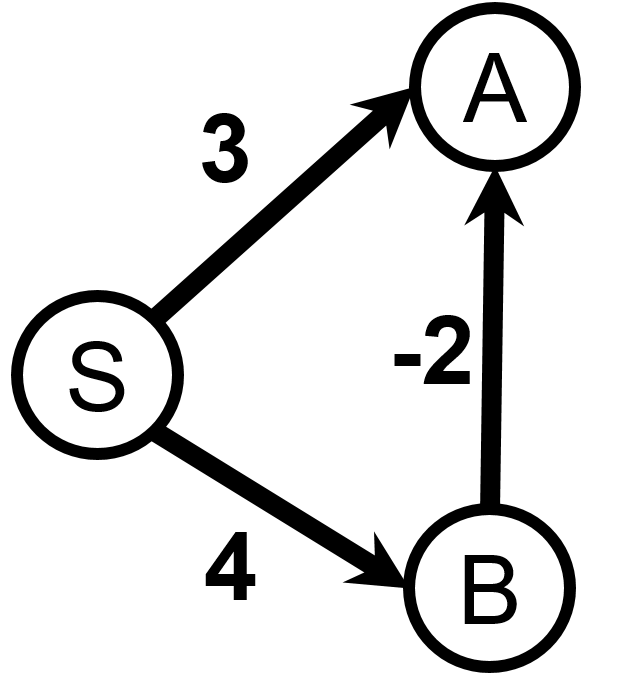
\includegraphics[width=0.2\textwidth]{2.png}
		\caption{\label{fig:problem2}Problem 2.}
	\end{figure}
	
	Problem 2 cannot be solved by Dijkstra's algorithm as it contains negative path weight. If we use Dijkstra's algorithm, we get \{S: 0, A: 3, B: 4\}, which is obviously wrong. In fact, the path S->B->A only cost 2, which is shorter than 3 obtained using Dijkstra's algorithm. Instead of locking vertices one by one, the Bellman-Ford algorithm evaluates all the path distances with edges adding up. 
	
	\subsection*{Step 1 to Problem 2}
	
	First assign 0 paths to the graph, and of course, the distance for S is 0, and $\infty$ for distances from S to A and to B, as shown in Figure~\ref{fig:problem2-step1}.
	
	\begin{figure}[htpb]
		\centering
		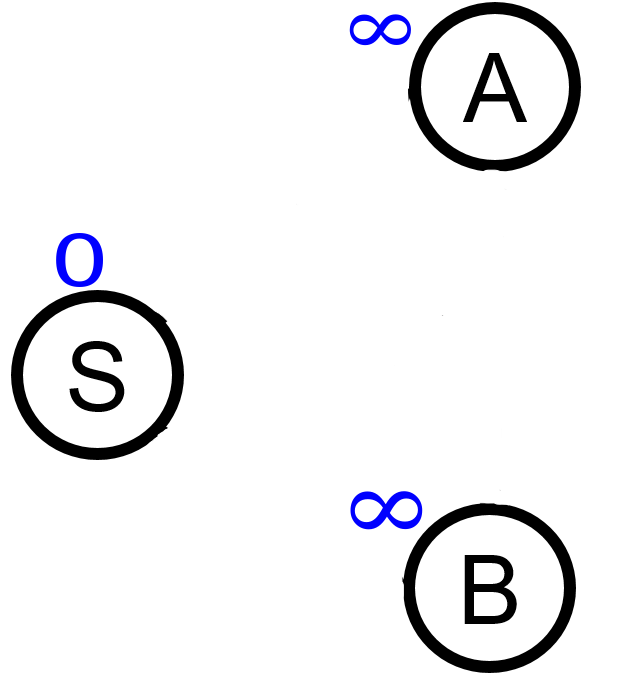
\includegraphics[width=0.2\textwidth]{2-1.png}
		\caption{\label{fig:problem2-step1}Step 1 to Problem 2, path lengths = 0.}
	\end{figure}
	
	\subsection*{Step 2 to Problem 2}
	
	As the path length 1 is applied, the distance from S to A is 3, and from S to B is 4, simply the same of their path weight. See Figure~\ref{fig:problem2-step2}.
	
	\begin{figure}[htpb]
		\centering
		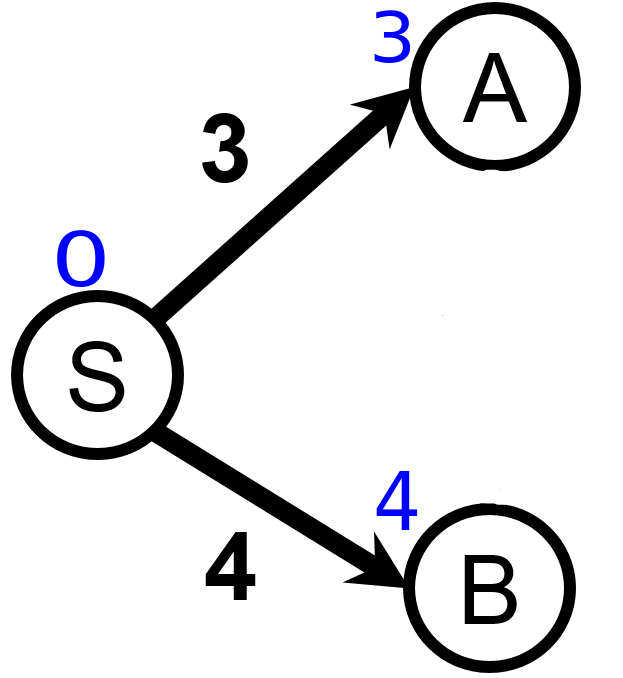
\includegraphics[width=0.2\textwidth]{2-2.png}
		\caption{\label{fig:problem2-step2}Step 2 to Problem 2, path lengths $\le$ 1.}
	\end{figure}
	
	\subsection*{Step 3 to Problem 2}
	
	When up to two path lengths are considered, S to A has a shorter choice: S->B->A, which is 4 -2 = 2. The result is shown in Figure~\ref{fig:problem2-step3}.
	
	\begin{figure}[htpb]
		\centering
		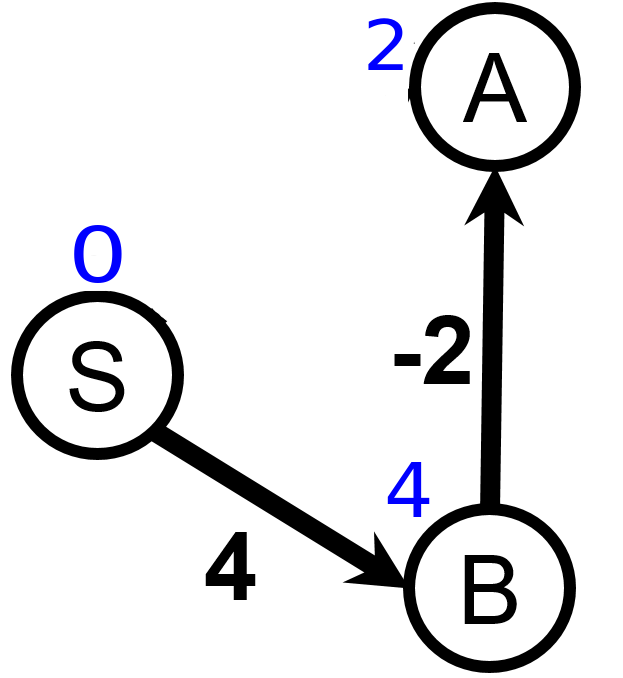
\includegraphics[width=0.2\textwidth]{2-3.png}
		\caption{\label{fig:problem2-step3}Step 3 (result) to Problem 2, path lengths $\le$ 2.}
	\end{figure}
	
	\subsection*{Result to Problem 2}
	
	Steps to problem 2 can be summarized in Table~\ref{tab:problem2-result}. 
	
	\begin{table}[htpb]
		\centering
		\begin{tabular}{lllll}
			Steps & Path lengths                 & S & A & B    \\ \cline{1-5} 
			1 & \multicolumn{1}{l|}{= 0} & 0 & $\infty$ & $\infty$ \\
			2 & \multicolumn{1}{l|}{$\le$ 1 } &0 & 3 & 4    \\
			3 & \multicolumn{1}{l|}{$\le$ 2} & 0 & 2 & 4   
		\end{tabular}
		\caption{\label{tab:problem2-result}Distances from S in problem 2.}
	\end{table}
	
	Figure~\ref{fig:problem2-step3} shows the shortest result graph to problem 2, and the shortest distances from S in problem 2 are \{S: 0, A: 2, B: 4\}.
	
	%    \bibliographystyle{IEEEtran}
	%    \bibliography{something}
	
	
\end{document}

%
% Please see the package documentation for more information
% on the APA6 document class:
%
% http://www.ctan.org/pkg/apa6
%